\section{Supplementary Materials}

% \begin{figure}[ht]
%     \centering
%     \begin{subfigure}{0.49\textwidth}
%         \centering
%         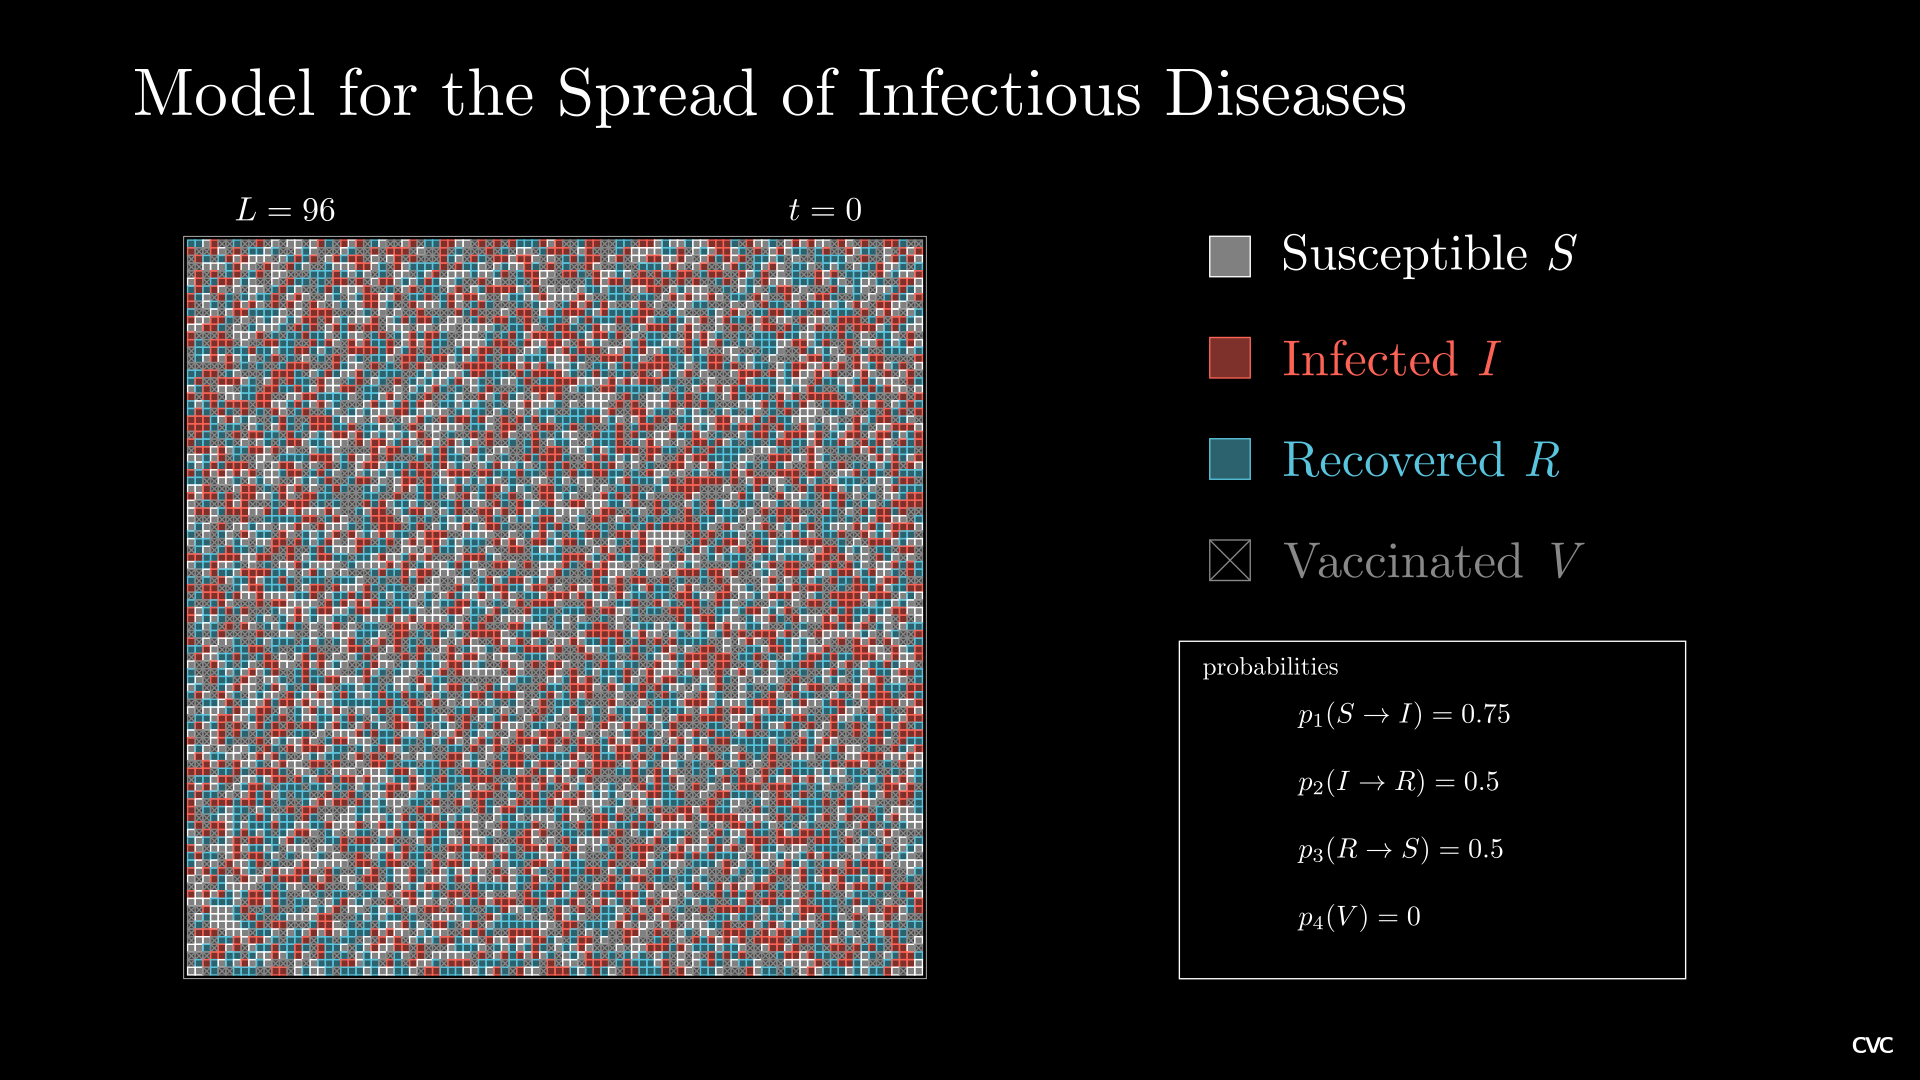
\includegraphics[width=1\textwidth]{images/soi_main_scene_75_50_50_25_init.png}
%         \subcaption{frame $t=0$}
%     \end{subfigure}
%     %\hspace{1cm}
%     \begin{subfigure}{0.49\textwidth}
%         \centering
%         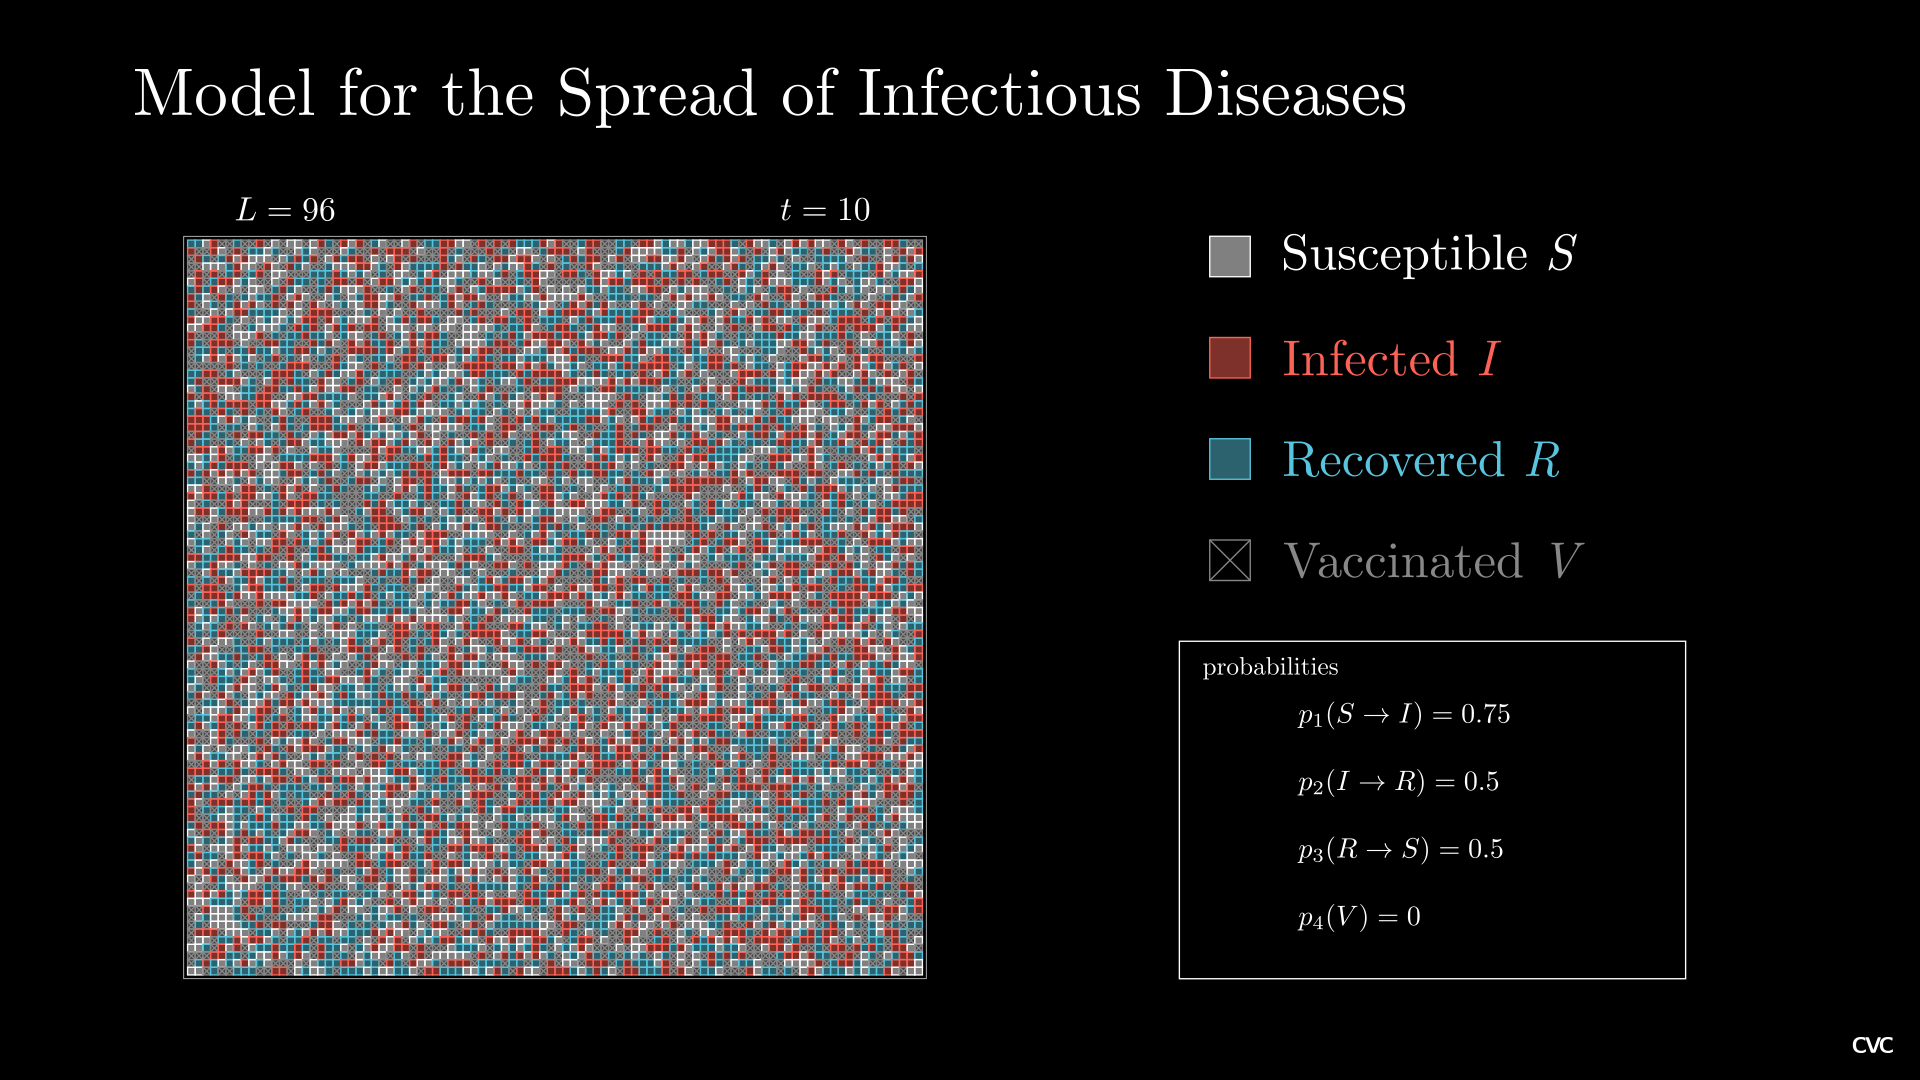
\includegraphics[width=1\textwidth]{images/soi_main_scene_75_50_50_25_t10.png}
%          \subcaption{frame $t=10$}
%     \end{subfigure}
%     \caption{Frames for simulation steps \textbf{(a)} $t=0$ and \textbf{(b)} $t=10$ of an animated simulation of the infectious disease model. The grid was initialized with a vaccination rate $p_4=0.25$
%     and progressed with the turnover probabilities $p_1=0.75$, $p_2=p_3=0.5$}\label{fig:Animation_Inf_t}
% \end{figure}

\begin{figure}[ht]
    \centering
    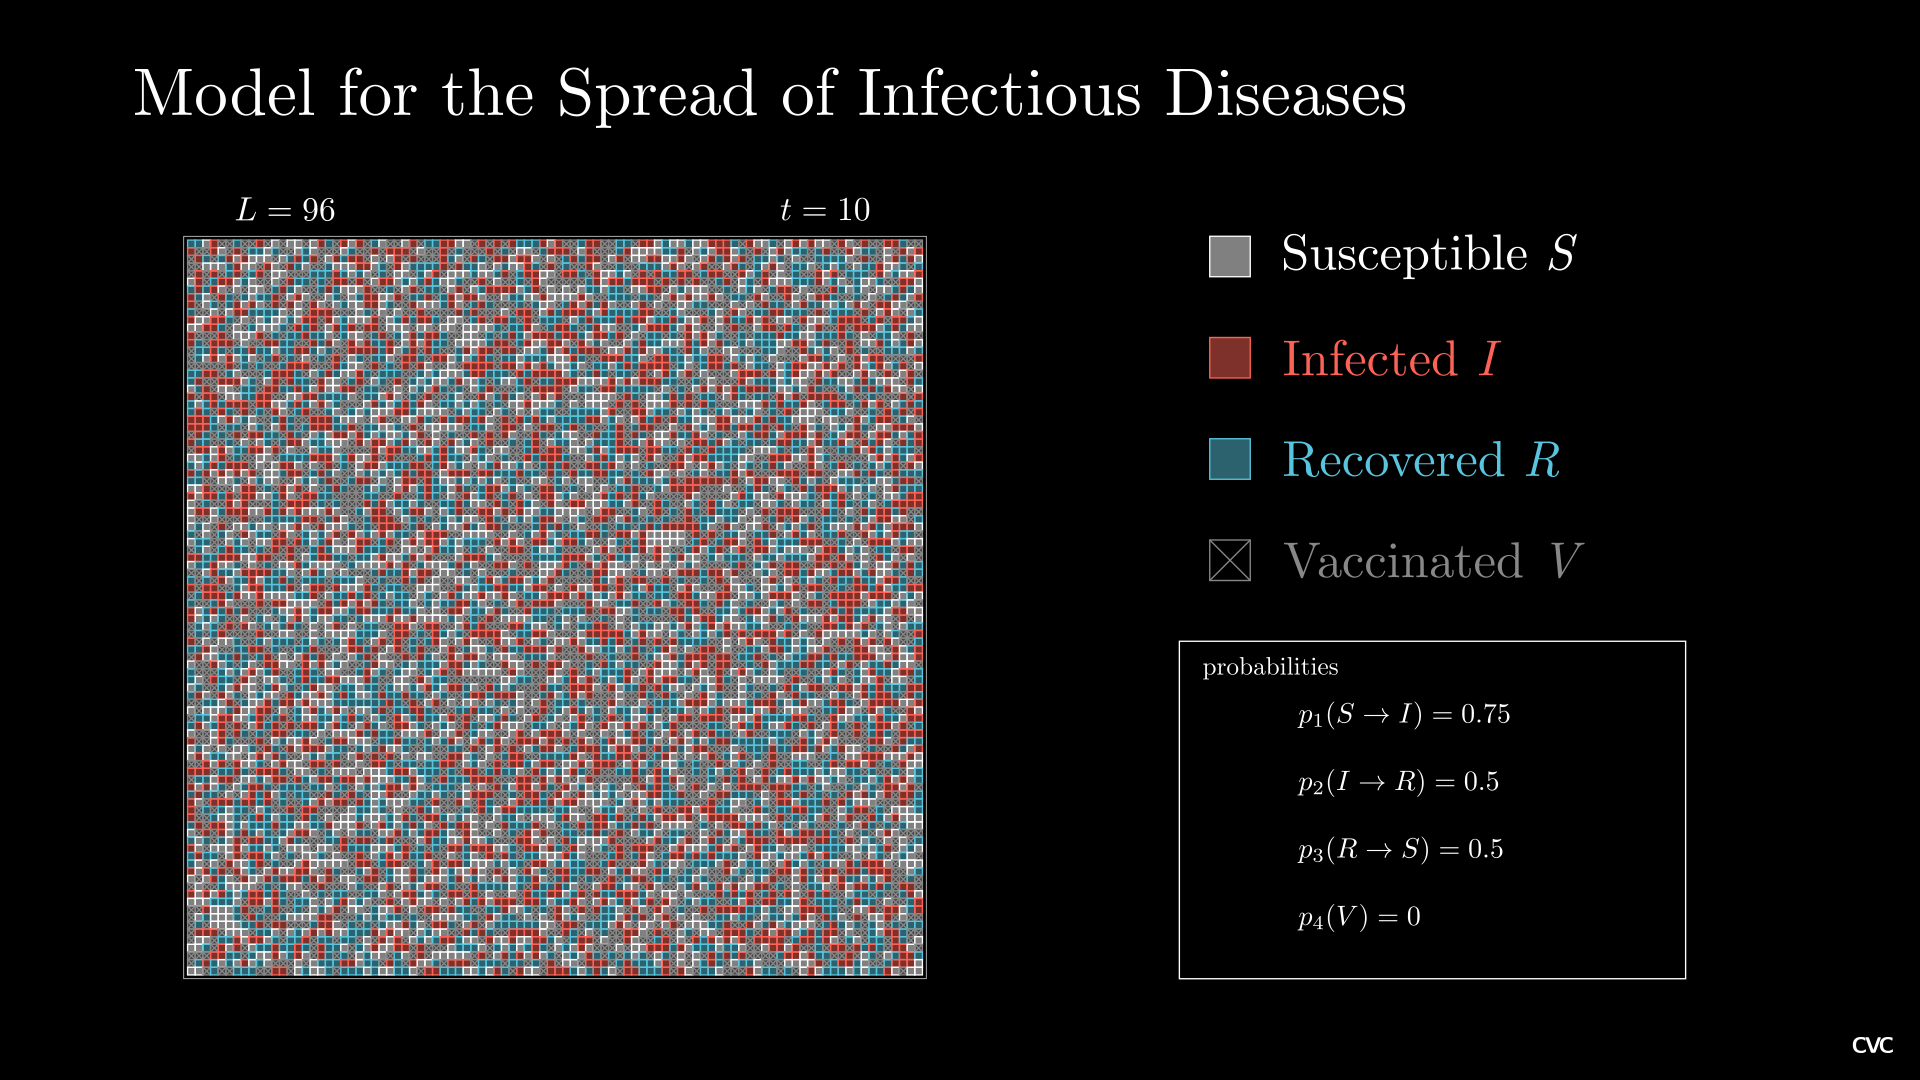
\includegraphics[width=1\textwidth]{images/soi_main_scene_75_50_50_25_t10.png}
    \caption{Frame $t=10$ of an animated simulation of the infectious disease model for the grid size $L=96$. The grid was initialized with a vaccination rate $p_4=0.25$ and progressed with 
    the turnover probabilities $p_1=0.75$ as well as $p_2=p_3=0.5$. The total animation as well as variations in the probabilities can be found under \texttt{/soi\_animations}.}\label{fig:apx_animation_inf_t}
\end{figure}